\documentclass[11pt]{article} % For LaTeX2e
\usepackage[utf8]{inputenc}
\usepackage{amsmath, amsfonts, amsthm, amssymb, algorithm, graphicx}
\usepackage{mathtools}
\usepackage{enumitem}
\usepackage{pdfpages}
\usepackage[noend]{algpseudocode}
\usepackage{fancyhdr, lastpage}
\usepackage[vmargin=1.20in,hmargin=1.25in,centering,letterpaper]{geometry}
\setlength{\headsep}{.10in}
\setlength{\headheight}{15pt}
 
% Macros
\DeclareMathOperator{\BigOm}{\mathcal{O}}
\newcommand{\BigOh}[1]{\BigOm\left({#1}\right)}
\DeclareMathOperator{\BigTm}{\Theta}
\newcommand{\BigTheta}[1]{\BigTm\left({#1}\right)}
\DeclareMathOperator{\BigWm}{\Omega}
\newcommand{\BigOmega}[1]{\BigWm\left({#1}\right)}
\DeclareMathOperator{\LittleOm}{\mathrm{o}}
\newcommand{\LittleOh}[1]{\LittleOm\left({#1}\right)}
\DeclareMathOperator{\LittleWm}{\omega}
\newcommand{\LittleOmega}[1]{\LittleWm\left({#1}\right)}

\newcommand{\calW}{\mathcal{W}}

\newcommand{\calY}{\mathcal{Y}}
\newcommand{\calS}{\mathcal{S}}
\newcommand{\calD}{\mathcal{D}}
\newcommand{\calN}{\mathcal{N}}

\newcommand{\calU}{\mathcal{U}}
\newcommand{\Alt}{\mathrm{Alt}}
\newcommand{\kl}{\mathrm{kl}}
\newcommand{\calA}{\mathcal{A}}
\newcommand{\calP}{\mathcal{P}}



\newcommand{\calH}{\mathcal{H}}

\newcommand{\ArgTop}{\mathrm{ArgTop}}
\newcommand{\Top}{\mathrm{Top}}
\newcommand{\TopEps}{\mathrm{Top}^{\epsilon}}
\newcommand{\ArgTopEps}{\mathrm{ArgTop}^{\epsilon}}


\newcommand{\KL}{\mathrm{KL}}
\newcommand{\Sym}{\mathrm{Sym}}
\newcommand{\Alg}{\mathrm{Alg}}
\newcommand{\Sim}{\mathrm{Sim}}


\newcommand{\istar}{i^*}
\newcommand{\im}{\mathrm{im }}
\newcommand{\Z}{\mathbb{Z}}
\newcommand{\C}{\mathbb{C}}
\newcommand{\R}{\mathbb{R}}
\newcommand{\I}{\mathbb{I}}
\newcommand{\Exp}{\mathbb{E}}
\newcommand{\Q}{\mathbb{Q}}
\newcommand{\sign}{\mathrm{sign\ }}
\newcommand{\abs}{\mathrm{abs\ }}
\newcommand{\eps}{\varepsilon}
\newcommand{\Var}{\mathrm{Var}}
\newcommand{\Cov}{\mathrm{Cov}}
\newcommand{\zo}{\{0, 1\}}
\newcommand{\SAT}{\mathit{SAT}}
\renewcommand{\P}{\mathbf{P}}
\newcommand{\NP}{\mathbf{NP}}
\newcommand{\coNP}{\co{NP}}
\newcommand{\co}[1]{\mathbf{co#1}}
\renewcommand{\Pr}{\mathbb{P}}
{
 \theoremstyle{plain}
      \newtheorem{asm}{Assumption}
}
\theoremstyle{plain}
\newtheorem{thm}{Theorem}[section]
\newtheorem{claim}[thm]{Claim}
\newtheorem{lem}[thm]{Lemma}
\newtheorem{cor}[thm]{Corollary}


\newtheorem{prop}[thm]{Proposition}

\theoremstyle{definition}
\newtheorem{defn}{Definition}[section]
\newtheorem{conj}{Conjecture}[section]
\newtheorem{exmp}{Example}[section]
\newtheorem{exc}{Exercise}[section]


\theoremstyle{remark}
\newtheorem*{rem}{Remark}
\newtheorem*{note}{Note}
\usepackage{mathtools}
\DeclarePairedDelimiter\ceil{\lceil}{\rceil}
\DeclarePairedDelimiter\floor{\lfloor}{\rfloor}

\makeatletter
\makeatother
\renewcommand{\theequation}{\arabic{section}.\arabic{equation}}
 
\algnewcommand\algorithmicinput{\textbf{INPUT:}}
\algnewcommand\INPUT{\item[\algorithmicinput]}
\algnewcommand\algorithmicoutput{\textbf{OUTPUT:}}
\algnewcommand\OUTPUT{\item[\algorithmicoutput]}
 
% Formatting Macros
 
%\pagestyle{fancy}
%\chead{\sc Problem \hmwkAssignmentNum.\hmwkProblemNum}
%\chead{}
%\rhead{\em Max Simchowitz}
\cfoot{}
\lfoot{}
\rfoot{\sc Page\ \thepage\ of\ \protect\pageref{LastPage}}
\renewcommand\headrulewidth{0.4pt}
\renewcommand\footrulewidth{0.4pt}

\newcommand{\qq}[1]{{\color{magenta}{(#1)}}}
\newcommand{\rb}[1]{{\color{red}{ #1}}}
\newcommand{\bl}[1]{{\color{blue}{ #1}}}
 
%%% magic code starts
%\mathcode`*=\string"8000
%\begingroup
%\catcode`*=\active
%\xdef*{\noexpand\textup{\string*}}
%\endgroup
%%% magic code ends

\title{Towards Controller Invalidation from Open- and Closed- Loop Experiments}

\author{Max Simchowitz\\
msimchow@berkeley.edu\\
Joint work with Qingqing Huang and Ross Boczar}


\begin{document}
\maketitle
\section{Introduction}
Broadly speaking, the aim of Robust Control is to design controllers which attain certain performance guarantees in the presence of systems disturbances, and plant misspecifications. For example, a cannonical problem is to design a linear controller $K$ so that for any misspecification $\Delta$ in a constraint-set $\boldsymbol{\Delta}$, the corresponding inter-connection loop is stable.


In order for robust synthesis to be possible, we require our knowledge about the uncertainty - e.g., the set $\boldsymbol{\Delta}$ -  to be pretty well specified. Indeed, for large enough families of uncertainty blocks, we may be unable to find practical controllers which stabilize all possible plants with those uncertainties. Hence, a natural net step might be to use \emph{experimental data} about the plant to learn additional constraints on the uncertainty blocks, in order to reach a tractable robust control problem.

On one extreme, one could try to essentially learn the entire plant behavior, up to a vanishingly small uncertainty. This problem is known as System Identification, or sys-id (see, for example~\cite{hardt2016gradient} and~\cite{shah2012linear}). Unfortunately, sys-id often performs poorly in practice, because a) dynamical are complex objects that require lots of data to pin down and b) restrictive a-priori models of plant behavior (e.g., linearity) make proper learner learning difficult. On the other extreme, the ``falsifiable control'' literature of \cite{jun1999automatic} at designing a controller by testing a sequences of candidate controllers $K_1,\dots,K_M$ in closed loop, and swapping out one controller to the next when the learner can certify that the current controller violates a certain performance specification. While this method does not rely on a-priori assumptions about plant structure, it seems too pessimistic in not taking advantage of plant modelling. Moreover, the methods do not offer any principled guidance on how to select from a a large, or possibly (uncountably) infite set of candidate controllers.

In this report, we will describe forthcoming work which tries to strike a middle ground between these two strategies. We will concern ourself with the relatively modest task of \emph{controller invalidation}, namely, using empirical open- and closed-loop data, how can we verify that a given controller $K$ fails to meet a certain performance objective? Ultimately, we hope that the invalidation problem will guide a principled and efficient approach to \emph{controller synthesis}, which is concerned with \emph{finding} a controller to achieve the desired performance guaranteed. However, since the sample complexity of the invalidation task is still not well known, we will restrict our inquiry to this more modest problem. In particular, we would like to know the following:
\begin{enumerate}
	\item How much open- and closed-loop data (and under what assumptions on those data) is required to invalidate a controller $K$? 
	\item What is the gap between computationally efficient invalidation procedures - such as those which rely on the $S$-procedure - and procedures which have access to unlimited computational power. 
\end{enumerate} 
We emphasize that this research is a work in progress. Thus, we will focusing on clarifying our initial steps, including the problem formulation, posing the problem as a non-convex quadratic program, relaxing the program via the S-procedure, and discussing challenges in proving sample complexity bounds going forward. Before continuing, we present a brief review of some statistical and data-driven approaches to learning dynamical systems, and designing controllers.

\section{Relevant Work}
Our approach is motivated by the model-invalidation work of\cite{smith2002nonlinear}, which uses experimental data about unknown plant to invalidate whether or not a set of candidate uncertainty $\Delta \in \boldsymbol{\Delta}$ is broad enough to account for observed plant behavior. Unlike the settings we will consider, their setting assumes that the uncertains may be nonlinear causal operators (though the nomimal plant is take to be linear). The system under consideration is thus described by the following LFT:
\begin{eqnarray}\label{LFTone}
\begin{bmatrix} y \\
z
\end{bmatrix} = \begin{bmatrix} P_{11} & P_{12} & P_{13} \\
P_{21} & P_{22} & P_{23}
\end{bmatrix}\begin{bmatrix} v \\
w \\
u
\end{bmatrix} \quad \text{and} \quad v = \Delta z
\end{eqnarray}
Here, the variables represent length $T$-signals, so for example $z \in \R^{n_zT}$. We assume that the signals $y$ and $u$ are known (measured), that $w$ is an unknown exogenous distribution which lies in a constraint set $\mathcal{H}_w$, and that $(z,v)$ are unknown un-measured internal signals which lie in the constraint set $\mathcal{H}_{ \boldsymbol{\Delta}} := \{z,v : v = \Delta z\}$. Given the observations $y$ and $u$, the goal is to understand
\begin{quote}
Do there exists disturbances $w \in \mathcal{H}_w$ and signals $(z,v) \in \mathcal{H}_{\Delta}$ which are consistent with the observations $(y,u)$, in the sense that Equation~\ref{LFTone} holds?
\end{quote}
In general, this problem is computationally infeasible for abitrary sets $\boldsymbol{\Delta}$. One step towards tractability is to express the uncertainty in terms of the intersections quadratic constraints of the form $\mathcal{H}_{w} = \{w: W_i(w) \ge 0\}_{1\le i \le d}$ and $\mathcal{H}_{\boldsymbol{\Delta}} = \{(z,v): Q_j(z,v) \ge 0 \}_{1 \le j \le r}$, where $W_i$ and $Q_j$ are \emph{quadratic functionals}, that is, functions of the form $F(x) = x^*Ax + b^*x + c$

One particular type of quadratic functional which is known to have great expressive power are IQC's, which given a signal $x(1),\dots,X(T)$ take the form $\sum_{t =1}^T F_t(x) \ge 0$ for quadratic functions $F_t(x)$ (thus the ``$F$'' matrix is block-diagonal). The seminal work on using IQC's to analyze feedback systems \cite{megretski1997system} establishes that many useful notions of constraints on both signals $w$ and pairs $(z,v)$ that arise from plants $\Delta \in \boldsymbol{\Delta}$ can be formalized in terms of IQC's, including bounded signal norms, sector-inequalities for non-linearities, and $l_2 \to l_2$ plant gains (or equivalently, $H_{\infty}$).
\subsection{Computational Infeasibility}
While describing the system in terms of quadratic contraints in general, and IQCs in particular, yields a clean problem formulation, verifying that the constraints have a non-empty intersection is, in-general, computationally intractable. The reason is that most interesting IQC's have indefinite ``$A$''-matrices, and thus their corresponding constraint sets are nonconvex (indeed, if a quadratic form $F$ has not $b$ and $c$ terms, then $F(x) \ge 0$ is trivially satisfied if $A \succeq 0$).

 Here, we present two IQC's of interest which express the sorts of constraints which will ultimately become important for our task. We will remark that both such constraints correspond to indefinite quadratic forms, thereby highlighting the computational difficulty of our task. The first is constraining the $l_2 \to l_2$ gain $\Delta$ by some $\gamma > 0$, that is, the constraint $\|v\|_2 \le \gamma \|z\|_2$. This can be expressed as the quadratic constraint
 \begin{eqnarray}
 Q_i(z,v) = \begin{bmatrix} z \\
 v \end{bmatrix}^* \begin{bmatrix} \gamma^2 I & 0 \\
 0 & - I \end{bmatrix}\begin{bmatrix} z \\
 v \end{bmatrix} \ge 0
 \end{eqnarray} 
 where we see immediately that the ``$A$'' term $\begin{bmatrix} \gamma^2 I & 0 \\
 0 & - I \end{bmatrix}$ is indefinite.

A second, more involved constraint is that the noise $w$ is essentially quite noise. One way of expressing this is that the correlation between $w(t)$ and $w(t+k)$ decreases as the delay $k$ increases. Assuming that $w(t)$ are scalars, we can express this condition as follows. Define the $k$-delayed autocorrelation
\begin{eqnarray}
r_w(t) = \frac{1}{T}\sum_{t=1}^{T} w(t + k \mod T)w(t)
\end{eqnarray}
Note that if $w(t)$ are i.i.d and zero-mean, then $r(0) \ge 0$ is an unbiased estimator of $\mathbb{Var}[w(t)]$. Hence, one definition of ``white'' is to say that that, for all $k \ne 0$, $|r_w(k)|$ is considerability smaller than its variance. That is,
\begin{eqnarray}\label{White}
|r_w(k)| \le \gamma r_w(0) \iff 
\end{eqnarray}
Letting $Z$ denote the cyclic shift operator on length-$T$ sequences, Equation~\ref{White} can be expressed as an IQC by the formula
\begin{eqnarray}\label{whiteIQC}
\gamma r_w(0) + \sigma r_w(k) = w^*(\gamma I + \frac{\eta}{2}((Z^k)^* + Z^k))w  \ge 0
\end{eqnarray}
where $k$ ranges from $1,\dots,T-1$, and $\eta \in \{-1,1\}$, yielding $2(T-1)$ quadratic constraints. Since $(Z^k)^* + Z^k)$ is indefinitely, it holds that the constraints in Equation~\ref{whiteIQC} are indefinite.

\subsection{A conservative solution: The S-procedure}
By lifting to the space of tuples $x = (w,v,z)$, our problem amounts to checking that the intersection of a finite collection of quadratic functional $\{G_i(x) \ge 0\}_{0 \le i \le r}$ is nonempty.  

A conservative approach to verifying the emptiness of the intersection, and thereby invalidating the model, is known as the $S$-procedure
\begin{lem} Suppose there exists scalars $\tau_i \ge 0$ such that
\begin{eqnarray}\label{eq:S-proc}
G_0 + \sum_{i=1}^r \tau_i G_i \ge 0
\end{eqnarray} Then, $\bigcap_{i=1}^r\{x:G_i(x) < 0\}\cap \{x: G_0(x) > 0\} =\emptyset$. 
\end{lem}
Note that the condition of Equation~\ref{eq:S-proc} amounts to checking if a linear form in $\tau$, subject to the nonnegativity constraints $\tau_i \ge 0$ in non-negative. By clever re-parametrization, this can then by represented as semi-definite program, which can be provably solved in polynomial time. 

\section{Adopting the IQC framework to Controller Invalidation}
In this section, we shall introduce our IQC framework for controller invalidation. In what follows, we have an unkown plant $P$, and our goal is to decide whether a closed loop system obtained by feeding back $K$ into $P$ satisfies certain performance guarantees. We will also work in the SISO setting, for the sake of simplicity, and assume all rollouts have length $T$. Finally, we will assume that $P$ is given as a finite impulse response $p$. As a block diagram, our system is represented as follows.
\begin{figure}[!ht]
  \centering
  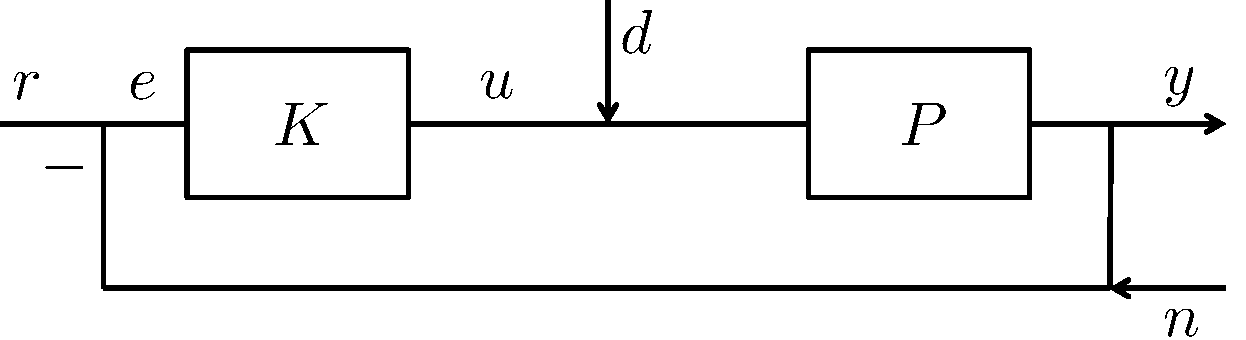
\includegraphics[width=.5\linewidth]{sys2.pdf}
\end{figure}
Our goal will be two invalidate $K$ using $N$ rollouts of open-loop data, and $M$ rollouts of closed loop data. For the open loop, we feed in an input $s$ into the plant $P$, and observe $v_i = Ps_i + w_i$, where $w_i$ is some noise. As a block diagram, 
\begin{figure}[!ht]
  \centering
  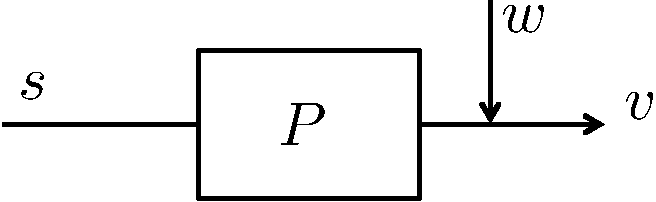
\includegraphics[width=.3\linewidth]{sys3.pdf}
\end{figure}
Assuming that $w_i$ satisfies lies in some constraint set $\mathcal{H}_w$, this induces the constraint that
\begin{eqnarray}
v_i - p_i * s_i \in \mathcal{H}_{w} 
\end{eqnarray}
where $*$ denotes the convolution operator. In other-words, if $T_{s_i}$ is the Toeplitz matrix associated with $s_i$, then, 
\begin{eqnarray}
v_i - T_{s_i} p_i  \in \mathcal{H}_{w} 
\end{eqnarray}
Since $v_i$ and $s_i$ are known, these amount to controls of the finite-impulse response of the plant $P$. 

Next, we perform $M$ closed loop experiments. From the block diagram, we find that
\begin{eqnarray}
y_j = p * (K (r_j - (y_j + n_j)) + d_j)
\end{eqnarray}
We will also assume that the disturbances $j$ and $d$ satisfy some regularity conditions, namely 
\begin{eqnarray}
d_j \in \mathcal{H}_{d} \quad \text{and} \quad n_j \in \mathcal{H}_n
\end{eqnarray}
Then, the invalidation step amount to asking whether or not the signal pairs $(d_j,y_j)$ and $(n_j,y_j)$ satisfy some performance guarantes. That is, 
\begin{eqnarray}
(d_j,y_i) \in \mathcal{H}_{(d,y)} \quad \text{and} \quad (n_j,y_j) \in \mathcal{H}_{(n,y)}
\end{eqnarray}
All in all, the following feasibility problem for all $i \in [n]$, 
\begin{align*}
  & (d_j,y_i) \in \mathcal{H}_{(d,y)} \quad \text{and} \quad (n_j,y_j) \in \mathcal{H}_{(n,y)} \quad \text{performance constraints}
  \\
  & y_j = p * ( K(r_j-(y_j+n_j)) +d_j), \quad\text{closed-loop constraint}
  \\
  & d_j \in \mathcal{H}_{d} \quad \text{and} \quad n_j \in \mathcal{H}_n \quad \text{disturbance and noise constraints}
  \\
  & v_i - T_{s_i}p \in \mathcal{H}_{w} \quad \text{open-loop constraints}
\end{align*}
In our case, we  will choose the sets $\mathcal{H}_{(\cdot)}$ to be specified by level-sets of indefinite quadratics, as in the previous section. Moreover, the closed loop constraint is in fact a bi-linear (and thus quadratic) constraint in the unkowns $p$, and in $n_j$ and $d_j$. Hence, we can write this constraint as the intersection of two quadratic inequality constraints, as shown below. This will leave us with a system of quadratic inequalities, which we can conservatively invalidate using the $S$-procedure.
\subsection{Representing the Closed Loop Constraint}
For $t = 1,\dots,T$, let $C_t$ denote the $t$-step convolution matrix, so that the convolution of signals $x_1 * x_2$ is given by $(x_1 * x_2)(t) = x_1^* C_tx_2$ (since $(x_1 * x_2)(t)$ is a bi-linear form in $x_1$ and $x_2$, such a $C_t$ is guaranteed to exist). Hence, if we define the variables $c_{t,j} = C_t K(r_j - y_j)$ (note that $r$ and $y$ are known), we can write the losed loop constraints as
\begin{align*}
   y_j(t) &= p^T C_t ( K(r_j-(y_j+n_j)) +d_j) \\
   &= p^T C_t K(r_j - y_j) + p^TC_t(d_j - Kn_j)\\
    &= p^T c_{t,j} + \begin{bmatrix} p \\
    d_j \\
    n_j \end{bmatrix}^T \begin{bmatrix} 0 & \frac{1}{2}C_t & \frac{-1}{2}C_t K  \\
    \frac{1}{2}C_t & 0 & 0 \\
     \frac{-1}{2}C_t K & 0 & 0 \\
     \end{bmatrix} \begin{bmatrix} p \\
    d_j \\
    n_j \end{bmatrix}
    &:= C_{t,j}(p,d_j,n_j)
\end{align*}
where we define the function $C_{t,j}(p,d_j,n_j)$ to be the quadratic form defined above.
\subsection{Constraints on Noise and Disturbance}
In general, it might be impossible to invalidate an ineffective controller from infinitely many observations. Indeed, the observation noise $w_j$ from the open loop ID is adversarially chosen, then it can greatly obfuscate our knowledge of $P$. Further still, if $d_j$ and $n_j$ are adversarially chosen, then they may chosen benigngly so that the observed closed loop data has the desired performance guarantees, will on ``typical'' sequences of noise and disturbances, the plant's performance guarantees might falter. 

Hence, for the aim of our statistical learning problem, we need to formulate some notion of what a ``typical'' disturbance/noise is. Then, we need to formulate a notion of a bad (i.e., falsifiable) controller based on typical sequences (indeed, a controller may actually attain the desired performance guarantees on some rare sequences but fail on average). Ultimately, our goal is to relate how ``bad'' a controller it is, to how frequently, and by how much, it fails performance guarantees on typical sequences of noises and disturbances. 

To this end, we shall assume that all of $w_i$, $n_j$ and $d_j$ are white Gaussian noise. Moreover, we will take our performance specification to be simple disturbance/noise rejection, that is,  $(y_j,d_j,r_j)$ (resp. $(y_j,n_j)$ must satisfy
\begin{eqnarray}\label{GainConstraint}
Q_{d}(y_j,d_j,r_j) &:=& \gamma_d^2\|d_j\|^2 - \|y_j - r_j\|^2 \ge 0 \quad \text{and} \\
Q_{n}(y_j,n_j) &:=& \gamma_h^2\|n_j\|^2 - \|r_j - y_j\|^2 \ge 0
\end{eqnarray}
Now, if we assumed that $n_j$ and $d_j$ were i.i.d white noise of known variances $\sigma_n^2$ and $\sigma_d^2$ , then $\|n_j\|^2$ and $\|d_j\|^2$ would concentrate tightly around $\sigma_n^2T$ (resp $\sigma_d^2T$). In other words, we could replace the $\gamma_d^2\|d_j\|^2$  in the above contraints with, say $(1+\epsilon)\sigma_d^2T$, and test approximately the same performance specification \emph{without having to guess $d_j$}. In this regime, we would therefore just want to run the controller $K$, and see how large the error $\|r_j-y_j\|$ becomes over the course of the trials,

However, the above example only takes place under very strong modeling assumptions that a) the noise is i.i.d and b) its variance is known. When the noise is unknown, and may vary with time, then the constraints in Equation~\ref{GainConstraint} become less vaccuous. 

The next step is to then characterize: what are the appropriate contraints to place on the $n_j$, $d_j$, and $w_i$ to enforce that they resemble ``white noise''? A simple small-energy ($l_2$) contraint
\begin{eqnarray}
\|n_j\|^2 \le T\sigma^2_n & \|d_j\|^2 \le T\sigma_d^2 & \|w_j\|^2 \le T\sigma^2_w
\end{eqnarray}
are a start, but these constraints do not preclude highly correlated, adversarially-chosen sequences of disturbances and observation noise which may interfere with inference. A more appropriate contraint may be ``average-uncorrelatedness'', in the sense of of the IQC from Section 2. Namely, defining the form 
\begin{eqnarray}\label{Qform}
Q_{\sigma,\eta,k}(w) =  w^T(\frac{\sigma}{\sqrt{T}} I + \frac{\eta}{2}((Z^k)^* + Z^k))w  
\end{eqnarray}
where $k \in \{1,\dots,T\}$, $\gamma > 0$ and $\eta \in \{-1,1\}$, and $Z$ is the $T\times T$ one-step cyclic shift operator.  Thus, we might impose contraints of the form
\begin{eqnarray}
Q_{\sigma_w,\eta,k}(w_i) \ge 0 &  Q_{\sigma_n,\eta,k}(n_j) \ge 0 &  Q_{\sigma_d,\eta,k}(d_j) \ge 0   
\end{eqnarray}
for $\eta \in \{-1,1\}$, and $k \in \{1,\dots,T\}$. Here, the $1/\sqrt{T}$ captures that the correlation between shifted-noise grow as the square-root of the time horizon $T$, whereas the unshifted auto-correlation should grow linearly in $T$. While this enforces that each rollout has uncorollated noise, it does not enforce the condition that successive rollouts are independent. This can be enforced as by considering the concatenations $\mathbf{w} = (w_1^T,\dots,w_N^T)^T$, $\mathbf{d} = (d_1^T,\dots,d_M^T)^T$, and $\mathbf{n} = (n_1^T,\dots,n_M^T)^T$ and imposing constraints of the form
\begin{eqnarray}\label{Qform}
Q_{\sigma,\eta,k}(\mathbf{w}_i) =  \mathbf{w}^T(\frac{\sigma}{\sqrt{NT}} I + \frac{\eta}{2}((\mathbf{Z}^k)^* + \mathbf{Z}^k))\mathbf{w} 
\end{eqnarray}
where $\mathbf{Z}$ is the shift operator on sequences of length $NT$.

\subsection{Least-Squares Based Confidence Intervals for Quadratic Constraint}
A more direct way to constraint $P$ is to create a least-squares confidence interval for the plant $p$. Here, let $\mathbf{v} = (v_1^T,\dots,v_N^T)^T$ denote the vector in $\R^{TN}$ of all open loop observations, and $\mathbf{w} = (w_1^T,\dots,w_N^T)^T$ the noise vector. Further, define
\begin{eqnarray}
T_{\mathbf{s}} = \begin{bmatrix} T_{s_1} \\
\dots\\
T_{s_N}
\end{bmatrix} \in \R^{NT \times T}
\end{eqnarray} 
Then,
\begin{eqnarray}
\mathbf{v} = T_{\mathbf{s}}p + \mathbf{w}
\end{eqnarray}
Hence, $p$ and the the least-squares estimator of $p$, $\widehat{p}$ are given by
\begin{eqnarray}
p = (T_{\mathbf{s}}^TT_{\mathbf{s}})^{-1}T_{\mathbf{s}}^T(\mathbf{v} - \mathbf{w}) \quad \text{and} \quad \widehat{p} = (T_{\mathbf{s}}^TT_{\mathbf{s}})^{-1}T_{\mathbf{s}}^T(\mathbf{v})
\end{eqnarray} 
so that $p - \widehat{p} = (T_{\mathbf{s}}^TT_{\mathbf{s}})^{-1}T_{\mathbf{s}}^T(\mathbf{w})$. Under the wide noise assumption, the error is then a Gaussian vector with covariance $(T_{\mathbf{s}}^TT_{\mathbf{s}})^{-1}T_{\mathbf{s}}^T(\mathbf{w}) \{(T_{\mathbf{s}}^TT_{\mathbf{s}})^{-1}T_{\mathbf{s}}^T(\mathbf{w})\}^T$, which can be used to provide quadratic confidence intervals on $p$ using concentration inequalities for non-isotropic Gaussians (e.g. Hanson-Wright\cite{rudelson2013hanson})

One could also consider regularizing $p$ to construct Lasso-based estimates, with potentially tighter confidence intervals. Indeed, constraining the FIR $p$ to have a small $l_1$ makes sense in the case that $P$ is an approximately-low order system, since then its coefficients should decay. This is another avenue we could investigate.

Finally, we remark that if the input matrix $(T_{\mathbf{s}}^TT_{\mathbf{s}})^{-1}T_{\mathbf{s}}^T(\mathbf{w})$ is sufficiently well conditioned, then as $N \to 0$, these Least-Squares and Lasso based estimators are consistent estimators of $p$. 



\section{Next Steps and Challenges}
At this stage, we have yet to formalize a condition on $K$ which we would expect to allow us to falsify it from finite data. $K$ should fail to meet performance specifications on ``typical data'', with some sort of margin. It is not clear if we will impose a condition that, with high probability on white noise $d_j$ and $n_j$, $K$ fails to meet performance standards, or simply with constant probability $K$ fails (thereby requiring many trials to observe the failure). 

Further still, we will run into the issue that, as we collect more data from a generative process, we become ever more likely to observe ``a-typical'' sequences of disturbances which may cause $K$ to fail, \emph{even if $K$ performs adequately on typical sequences}. Thus, we may need to formulate a notion of strong performance on most trials (which is often computationally hard), or work with notions of average performance over rollouts (which are considerably weaker and thus harder to falsify). 

Finally, once the correct assumptions are put in place, we need to understand the sampled complexity of the $S$-procedure in invalidating such a model. One open question is that, while a controler $K$ should be able to be invalidated in the limit of infinite rollouts (indeed, assuming stochastic noise, you can learn $P$ to arbitrary high precision, and use standard robust control-theoretic tools to evaluate its performance), the over-conservative $S$-procedure may not even be statistically consistent!







\bibliographystyle{plain}
\bibliography{invalid}
\end{document}	